%%%%%%%% ICML 2021 EXAMPLE LATEX SUBMISSION FILE %%%%%%%%%%%%%%%%%

\documentclass{article}

% Recommended, but optional, packages for figures and better typesetting:
\usepackage{microtype}
\usepackage{graphicx}
\usepackage{subfigure}
\usepackage{booktabs} % for professional tables
\usepackage{gensymb}
\usepackage{amsmath}
\usepackage{physics}
\usepackage{amssymb}

% hyperref makes hyperlinks in the resulting PDF.
% If your build breaks (sometimes temporarily if a hyperlink spans a page)
% please comment out the following usepackage line and replace
% \usepackage{icml2021} with \usepackage[nohyperref]{icml2021} above.
\usepackage{hyperref}

% Attempt to make hyperref and algorithmic work together better:
\newcommand{\theHalgorithm}{\arabic{algorithm}}

% Use the following line for the initial blind version submitted for review:
%\usepackage{icml2021}

% If accepted, instead use the following line for the camera-ready submission:
\usepackage[accepted]{icml2021}

% The \icmltitle you define below is probably too long as a header.
% Therefore, a short form for the running title is supplied here:
\icmltitlerunning{Stat157: Information Theory Final Project}

\begin{document}

\twocolumn[
\icmltitle{An Emperical Study of Phase Transitions in the Ising Model}

% It is OKAY to include author information, even for blind
% submissions: the style file will automatically remove it for you
% unless you've provided the [accepted] option to the icml2021
% package.

% List of affiliations: The first argument should be a (short)
% identifier you will use later to specify author affiliations
% Academic affiliations should list Department, University, City, Region, Country
% Industry affiliations should list Company, City, Region, Country

% You can specify symbols, otherwise they are numbered in order.
% Ideally, you should not use this facility. Affiliations will be numbered
% in order of appearance and this is the preferred way.
\icmlsetsymbol{equal}{*}

\begin{icmlauthorlist}
\icmlauthor{Leon Ma}{to}
\end{icmlauthorlist}

\icmlaffiliation{to}{Department of Statistics, UC Berkeley}

\icmlcorrespondingauthor{Leon Ma}{lma00@berkeley.edu}

% You may provide any keywords that you
% find helpful for describing your paper; these are used to populate
% the "keywords" metadata in the PDF but will not be shown in the document
\icmlkeywords{Machine Learning, ICML}

\vskip 0.3in
]

% this must go after the closing bracket ] following \twocolumn[ ...

% This command actually creates the footnote in the first column
% listing the affiliations and the copyright notice.
% The command takes one argument, which is text to display at the start of the footnote.
% The \icmlEqualContribution command is standard text for equal contribution.
% Remove it (just {}) if you do not need this facility.

\printAffiliationsAndNotice{}  % leave blank if no need to mention equal contribution
%\printAffiliationsAndNotice{\icmlEqualContribution} % otherwise use the standard text.

\begin{abstract}
    Ising models have traditionally been solved with Markov chain Monte Carlo methods, 
    the most popular of which is the Gibbs’ sampler. However, MCMC suffers from correlated samples and long mixing times. 
    In recent years, a new class of algorithms based on variational inference has come to light. These algorithms promise faster convergence abit at the cost of convergence. 
    Belief propagation is an inference algorithm that uses message passing in order to approximate the probability distribution over a factor graph. 
    In this paper, we apply belief propagation to solve the Ising model and show that during belief propagation, the 2D Ising model exhibits a phase transition similar to simulations using MCMC. We compare metrics of phase transitions to MCMC approaches and known theoretical results and conclude that belief propagation can solve the Ising model to a high degree of accuracy and retain many interesting properties that the Ising model is known for. 
\end{abstract}

\section{Introduction}
\label{Introduction}
    The Ising model is a mathematical model of ferromagnestim in statistical mechanics.
    Invented first by Wilhelm Lenz in 1920 and the equations of the one-dimensional Ising model were solved in by
    Lenz's student Ernst Ising in 1924. In 1944, Lars Onsager solved the equations for the two-dimensional case. 
    As of today, no analytic solution has been found in dimensions three or higher. Over the last 100 years, many other problems such as percolation, min cut max flow, error correction, neural networks, and neurodegenerative diseases were
    shown to be very closely mathematically related to the Ising model. 
    The Ising model's relatively simple formulation yet rich and general mathematical properties makes a \textit{drosophila} of physics, mathematics, statistics, and computer science.

    Since Onsager's solution, it is known that the Ising model exhibits a phase transition just like magnets in the real world. Above the
    a special temperature, the critical temperature (or more generally the critical point), the system under goes a rapid change, changing from an ordered magnetic state to a disordered non-magnetic state. 
    This rapid change of order is fundementally related to the relationship between energy, entropy and free energy. When the system is at the critical point, it is said to be at
    criticality and many interesting properties such as scale invariance and long range correlations are present
    during the phase transition. 

    However, due to the difficulty of solving the Ising models in higher dimensions, many approxiomation methods have been devolved over the years. 
    Statistical physicists developed mean field theory and the cavity method to find approximate analytic solutions. In more recent times, the rise of computational 
    power allowed computer algorithms to approximate solutions to the Ising model. The most well known class of algorithms are Markov Chain Monte Carlo (MCMC) algorithms such as 
    Metropolis-Hasting algorithm and Gibbs' sampling. Although these algorithms are powerful and still widely used, they suffer long convergence times and autocorrelated samples.
    
    In this paper, we explore an alternative algorithm to approximately solve the Ising model called belief propagation. Belief propagation works by sending messages 
    from each node of a factor graph to iteratively find the probability distrubition. We show that this method can calculate solutions comparable to Metropolis-Hastings and Gibbs sampling 
    and show that solutions given by belief propegation exhibit a phase translation like predicted theoretically. 


\section{Background}
\label{Mathematical Background}
    \subsection{Ising Model}
    The Ising model models ferromagnestic materials as a two-dimensional lattice where each lattice site represents an 
    electron that is either spin up $\sigma_i = +1$ or spin down $\sigma_i = -1$. Each lattice point only interacts
    with it's adjacent neighbors. In this paper, we impose periodic boundary conditions. This is equivalent to the lattice wrapped around the surface of a torus. This simulates 
    an infinitely large lattice and midigates boundary effects. 
    
    \begin{figure}[ht]
        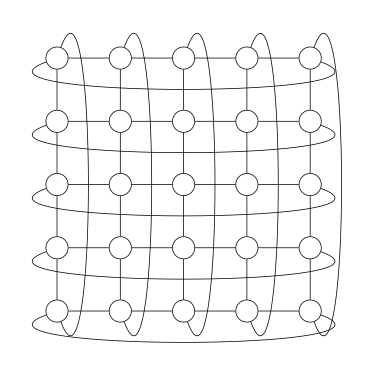
\includegraphics[width=\columnwidth]{diagrams/loopy_ising_model.png}
        \caption{Ising Model with Periodic boundary conditions}
        \label{fig:1}
    \end{figure}
    
    
    Thus, the total energy (also known as the Hamiltonian $H$ in physics literature) is
\begin{equation}
    E(\sigma) = - J \sum_{(i,j) \in \mathcal{N}} \sigma_i \sigma_j - B \sum_{j} \sigma_j
\end{equation}
where $(i,j) \in \mathcal{N}$ is understood to be the sum over all pairs of $(i,j)$ that are adjacent neighbors,
$J$ is the physical constant knows as the coupling strength and $B$ is the strength of the external magnetic field.
We assume $J=1$ for simplicity and no external magnetic field $B=0$. Then our total energy is
\begin{equation}
    E(\sigma) = - \sum_{(i,j) \in \mathcal{N}} \sigma_i \sigma_j 
\end{equation} 
We notice that the energy is lower when $\sigma_i$ and $\sigma_j$ are the same sign and greater when $\sigma_i$ and $\sigma_j$ 
are different signs. The energy is minimized when the spins are alligned in the same direction, corresponding to a magnetized state.
However, the entropy is maximized when the spins are misalligned corresponding to a demagnetized state.

We can then introduce the partition function, 

\begin{equation}
    Z = Z(\beta) = \sum e^{-\beta E(\sigma)}
\end{equation}

The PMF of the system is given by the Boltzmann distribution

\begin{equation}
    P(\sigma) = \frac{e^{-\beta E(\sigma)}}{Z}
\end{equation}

where the inverse temperature $\beta = 1/(kT)$, $k$ is Boltzmann's constant, and the partition function $Z$ is the normalization constant.
Given an initial square lattice of $\sigma$ and inverse temperature $\beta$ the goal is to find the equalibrium distrubition over $\sigma$.


\subsection{Phase Transition}
In physics a phase transition refers to a change of a system from one state to another. A classical example is ice melting into water.
However, more generally it refers to the rapid change of a systems order parameter as a function of one or more of the systems parameters. 
This more general defintion can be applied to other fields such as rate distortion theory. The Ising model predicts a phase transition of a ferromagnetic system like an iron magnet from a demagnetized state to a magnetized state. 
It is known emperically that heating a magnet above a certain temperature known as the Curie temperature (770 \degree C for iron) causes rapid
demagnetization. The characteristic feature of the phase transition is that the magnetization strength changes very rapidly over a short range of temperature
similar to how ice melts into water over a narrow temperature of range of 0\degree C. This transition from order to disorder is due to the changing strength of
energetic and entropic forces.

In nature, systems tend to minimize a thermodynamic quanity known as free energy. The free energy is given by

\begin{equation}\label{eq:eq1}
    F = E - TS
\end{equation}
where $S$ is the thermodynamic entropy. At high temperatures the entropy term is dominant and at low temperature the energetic term is dominant.
This explains why the spins are misalligned at high temperature. The thermal energy from the envirnoment is sufficent to flip the lattice site spins.
This thermal function acts like a corrupting force constantly distrupting the spins of the system. It is also convient to define the free energy as

\begin{equation}
    F = kT \ln Z
\end{equation}

These two formulas are equivalent


\begin{align}
    S &= -k \sum_i p_i \ln p_i \\
    &= -k \sum_i \frac{e^{-\beta E_i}}{Z} \ln \left(\frac{e^{-\beta E_i}}{Z} \right) \\
    &= -k \sum_i \frac{e^{-\beta E_i}}{Z} (-\beta E_i - \ln Z) \\
    &= k \beta \sum_i \frac{e^{-\beta E_i}}{Z} E_i + k \sum_i \frac{e^{-\beta E_i}}{Z} \ln Z \\
    &= k \beta \langle E \rangle + k \ln Z \\
    &= k \beta E + k \ln Z
\end{align}

since the energy $E$ is simply the energy averaged all over microstates $\langle E \rangle$. 
Plugging this into \eqref{eq:eq1} yields

\begin{align}
    F &= E - T (k \beta E + k \ln Z) \\
    &= E - T (k \frac{1}{kT} E + k \ln Z) \\
    &= E - E + kT \ln Z \\
    &= kT \ln Z
\end{align}

The energy can also be defined in terms of the partition function as

\begin{align}
    E &= -\pdv{\ln Z}{\beta} \\
    &= -\frac{1}{Z} \frac{Z}{\beta} \\
    &= -\frac{1}{Z} \pdv{}{\beta} \sum_i e^{-\beta E_i} \\
    &= -\frac{1}{Z} \sum_i -E_i e^{-\beta E_i} \\
    &= \sum_i E_i \frac{e^{-\beta E_i}}{Z} \\
    &= \langle E \rangle \\
    &= E 
\end{align}

These equations will be relevant when we discuss the connection between belief propagation and minimization of the Bethe free energy.

By analyizing at what temperature the energy and entropy terms balance, Onsager solved the 2D Ising model analytitically in the case of no external magnetic field and showed that the critical temperature is

\begin{equation} \label{eq:eq24}
    T_c = \frac{2J}{k \ln(1 + \sqrt2)}
\end{equation}
or in terms of $\beta_c = \frac{\ln(1 + \sqrt2)}{2J}$. This derivation is very technical and will not be covered here.




Systems at the critical point exhibits many interesting properties. The first is the rapid change of the order parameter.
In the case of the Ising model, the order parameter is the magnetization given the average value of the spins.

\begin{equation}
    \langle m \rangle = \frac1N \sum_{i=1}^N \sigma_i
\end{equation}

In order to not give preference to major spin down or spin up configurations, it is convient to define the mangetization squared
$\langle m^2 \rangle = \frac1N \sum_{i=1^N} \sigma_i^2$.

At the critical temperature, the system reaches a critical state where order and disorder are perfectly matched.
Here, the model exhibits long range correlations not found at other temperature reigmes. The Ising model only takes into account
interactions between neigboring lattice sites. Therefore, we expect the correlation between lattice sites to be very short and lattice sites
long distances apart to act inpendendently. This is in general true except when the system is at criticality. When order and disorder
are perfectly balanced, local interactions have a ripple effect, meaning that local interactions lead to long range communication. The correlation function is given by

\begin{equation}
    C_{i,j} = \langle (\sigma_i - \langle \sigma_i \rangle)(\sigma_j - \langle \sigma_j \rangle) \rangle
\end{equation}

where $\langle \cdot \rangle$ denotes the time average. Then we can define the correlation length function,

\begin{equation}
    C(d) = \mathbb{E} \left[ C_{i,j} \mid D(i,j) = d \right]
\end{equation}

which is the correlation strength as a function of the distance between lattice sites.

Another interesting phenomona observed at criticality is scale invariance. Suppose for each 3 by 3 block of spins, we replace that block
with the spin corresponding to the majority spin value out of those 9 smaller spins. Apply this procedure to the whole lattice and we have
a new lattice with a third of the distance scale. This procedure is called a course graining. We can continue this procedure indefinitely on an 
infinitely large lattice. At the critical point, all these lattices of varying length scales look the same, in other words there is no 
characteristic scale. To show this idea graphically, we plot the distribution of the cluster sizes where a cluster is a group of lattice points with
the same spin. This gives us a scaling equation 

\begin{equation}
    \frac{f(kx)}{f(x)} = g(k)
\end{equation}

where $f(x)$ is the probability of observing a cluster size with size $x$ and $k$ is a scaling factor.
Suppose $k=3$. Then this tells us that the probability of observing a cluster three times larger then $x$
is a function $g(k)$. It turns out that we can show the only function $g$ that satifies this property is
$g(k) = k^{-\gamma}$ for some constant $\gamma$ which means


\begin{equation}
    f(x) = A x^{-\gamma}
\end{equation}

This is a power law. We can visualize this as a straight line on a log-log plot $\log f(x) = -\gamma \log x + \log A$.
The slope of such line on a log-log plot is $-\gamma$.
 
\section{Methods}
\label{Methods}

\subsection{Metropolis-Hasting}
In the previous sections we have described the mathematical background behind the Ising model and theory of phase transitions.
However, solving the Ising model analytitically is extremely difficult and in practice computational methods are used. The most common of these methods 
are Monte Carlo Markov Chain methods. The simpliest example of MCMC is the Metropolis-Hasting algorithm. Metropolis-Hasting works by building 
an implict Markov Chain model of the system and sampling from the stationary distrubtion of the chain to generate samples of the system's true probability
distrubtion. This works because when the Ising model is at thermodynamic equalibrium, it's Markov chain satifies the detailed balance equations

\begin{equation}
    \pi_{\mu} P(\mu \rightarrow \nu) = \pi_{\nu} P(\nu \rightarrow \mu)
\end{equation}

where $\mu$ and $\nu$ are states, $p_{\mu}$ is the probability that the system is in state $\mu$ and $P(\mu \rightarrow \nu)$
is the probability that the system will transition from state $\mu$ to state $\nu$. Then we have that 

\begin{align}
    \frac{P(\mu \rightarrow \nu)}{P(\nu \rightarrow \mu)}
    &= \frac{\pi_{\nu}}{\pi_{\mu}} \\
    &= \frac{e^{-\beta E_{\nu}} / Z}{e^{-\beta E_{\mu}} / Z} \\
    &= e^{-\beta(E_{\nu} - E{\mu})} \\
    &= e^{-\beta \Delta E}
\end{align}

where the change in energy $\Delta E = E_{\nu} - E{\mu}$. Suppose that we start in state $\mu$. At each step of the algorithm, we flip a random spin $\sigma_j \mid j \sim U\{1,2,\ldots,n\}$ to create a new state $\nu$.
If $E_{\nu} < E_{\mu}$ then $\Delta E < 0$ and the system would enter the lower energy state so $P(\nu \rightarrow \mu) = 1$. This gives us
$P(\mu \rightarrow \nu) = e^{-\beta \Delta E}$. Note that the probability that the system moves to a higher energy state 
is non zero due to random fluctuations due to the thermal energy. Furthermore as $T$ increases, $\beta$ decreases causing $e^{-\beta \Delta E}$
to increase meaning that spin flips are more likely at higher temperature. If $E_{\mu} < E_{\nu}$ we can similarly define $P(\mu \rightarrow \nu) = 1$
and $P(\nu \rightarrow \mu) = e^{-\beta(-\Delta E)}$. This gives us the acceptance probability for $\mu \rightarrow \nu$ to be

\begin{equation}
    \alpha = \min(1, e^{-\beta \Delta E})
\end{equation}

Thus, we only need to calculate the difference in energy $\Delta E = E_{\mu} - E_{\nu}$ when determining wether to accept or reject a canidate state.
However, as we'll see, this naive method of randomly flipping a spin can lead to pathelogical a Markov chain.

\subsection{Gibbs Sampler}
The Gibbs sampler begins with $\mathbf{X} = (x_1, \ldots, x_2)$ with joint distribution $p(x_1, \ldots, x_n)$. Denote the $i$th sample
$\mathbf{X}^{(i)} = (x_1^{(i)}, \ldots, x_n^{(i)})$. Then the Gibbs sampler samples

\begin{equation} \label{eq:eq33}
    x_j^{(i+1)} \sim P(x_j^{(i+1)} \mid x_1^{(i+1)}, \ldots, x_{j-1}^{(i+1)}, x_{j+1}^{(i+1)}, \ldots, x_{n}^{(i+1)})
\end{equation}

In our specific case we choose the index $j \sim U\{1,2,\ldots, n\}$. $x_j^{(i+1)}$ is given by $\ref{eq:eq33}$ and 
$x_{\backslash j}^{(i+1)} = x_{\backslash j}^{(i)}$. The advantage of Gibbs sampling is that in some cases is it simpler ot sample from the conditional
distrubtion then it is to marginalize the joint distrubtion.

In the case of our Ising model, at each time step we sample a lattice point $j$ uniformly. Then according to our update rule, 
the probability of $\sigma_j$ being spin up is given by 

\begin{equation}
    \begin{split}
    &P(\sigma_j = +1) = \\
    &\quad \frac{\exp(-\beta E(\ldots, \sigma_j = +1, \ldots))}{\exp(-\beta E(\ldots, \sigma_j = +1, \ldots)) + \exp(-\beta E(\ldots, \sigma_j = -1, \ldots))}
    \end{split}
\end{equation}

where $\ldots$ denotes the spins of the other lattice points at the previous time step. $P(\sigma_j = -1)$ is given similarly. 
Notice that this update rule does not depend on the value of $\sigma_j$ at the previous time step. This update rule
is referred to as the heat bath update rule because the orientation of each spin depends only on the energy transferred from the thermal energy of the heat bath.

Now lets try to reformulate this update rule to better match our Metropolis-Hasting update rule. 
Suppose that initially $\sigma_j = -1$. Let the event that $\sigma_j = +1$ at the next time step be denoted $\mu \rightarrow \nu$ as before.
Then 
\begin{align}
    &P(\mu \rightarrow \nu) = P(\sigma_j = +1) = \\
    &\frac{\exp(-\beta E(\ldots, \sigma_j = +1, \ldots))}{\exp(-\beta E(\ldots, \sigma_j = +1, \ldots)) + \exp(-\beta E(\ldots, \sigma_j = -1, \ldots))} \\
    &= \frac{\exp(-\beta E_{\nu})}{\exp(-\beta E_{\nu}) + \exp(-\beta E_{\mu})} \\
    &= \frac{\exp(-\beta (E_{\mu} + (E_{\nu} - E{\mu})))}{\exp(-\beta (E_{\mu} + (E_{\nu} - E{\mu}))) + \exp(-\beta E_{\mu})} \\
    &= \frac{\exp(-\beta (E_{\mu} + \Delta E))}{\exp(-\beta (E_{\mu} + \Delta E)) + \exp(-\beta E_{\mu})} \\
    &= \frac{\exp(-\beta E_{\mu}) \exp(-\beta \Delta E)}{\exp(-\beta E_{\mu}) \exp(-\beta \Delta E) + \exp(-\beta E_{\mu})} \\
    &= \frac{\exp(-\beta \Delta E)}{\exp(-\beta \Delta E) + 1} \\
    &= \frac{1}{1 + \frac{1}{\exp(-\beta \Delta E)}}
\end{align}
Following the same derivation for the probability that $\sigma_j$ is initially at spin up then is flipped spin down gives the same expression.
Thus, the probability of the spin flip under the heat bath update rule is 

\begin{equation}
    \alpha = \left(1 + \frac{1}{\exp(-\beta \Delta E)}\right)^{-1}
\end{equation}

We can just replace our Metropolis-Hasting algorithm with this new acceptance probability showing that the Gibbs sampler is special case of the Metropolis-Hasting algorithm. 
This class of update rules that depend soley on the Boltzmann distrubtion is known as Glauber dynamics. We shall see in practice this update rule generally results in faster convergence.


\section{Experiments}
\subsection{MCMC Convergence}
    First we will compare the convergence of the Metropolis-Hasting sampler to the Gibbs sampler.

    We see that Gibbs sampler has faster convergence and is more stable then the Metropolis-Hasting sampler. Thus, in the future,
    we will be using the Gibbs sampler.
\subsection{Order Parameters}

Now we study how the energy and the magnetization change with $\beta$ and the lattice size $L$. 
Both the energy and magnetization tells us how ordered our lattice is. Recall that when our lattice has
has most of the spins pointing in the same direction, these aligned spins create favorable energetic interactions
leading to the lattice being in a lower energy state.

\begin{figure}[ht]
    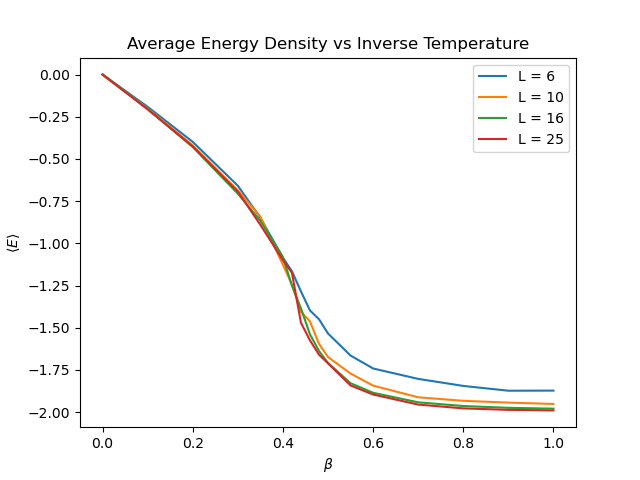
\includegraphics[width=\columnwidth]{plots/avg_energy_vs_beta.png}
    \caption{Average Energy Density vs Inverse Temperature}
    \label{fig:3}
\end{figure}

We notice that as $\beta$ decreases, $T$ increases and thus the thermal energy distrupts the orientation of the spins, causing
the energy of the system to increase as $\beta$ decreases. This is more appearent when we observe the plot of the magnetization.

\begin{figure}[ht]
    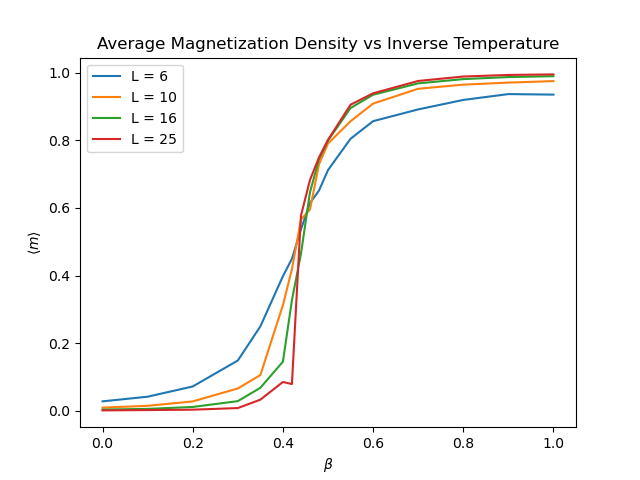
\includegraphics[width=\columnwidth]{plots/avg_mag_vs_beta.png}
    \caption{Average Magnetization Density vs Inverse Temperature}
    \label{fig:4}
\end{figure}

We see that the magnetization looks like $\langle m \rangle \sim \mathrm{arcsinh}(\beta)$ as predicted by theory. 
Furthermore, the critical $\beta$ seems to be around 0.44. Comparing this experimental observation to Onsager's solution given 
in \eqref{eq:eq24} gives 
\begin{equation}
    \beta_c = \frac{\ln(1+\sqrt{2})}{2} \approx 0.4407
\end{equation}
which is in very close agreement. 

Lastly we also notice that as $L$ increases, the phase transition becomes sharper. This suggests that phase transitions are
an emergent phenomenon. In reality, the number of electrons is orders of magnetudes larger then this simulation giving the extremely sharp 
phase transitions we observe in nature.

\subsection{Critical Phenomena}
Now we turn to special properties of the Ising model at criticality. As we outlined in section 2.2, systems at criticality
exhibit long range correlations. Using $L=16$ and $p=0.5$ we plot the correlation strength as a function of the distance $d$ between
two lattice points. 

\begin{figure}[ht]
    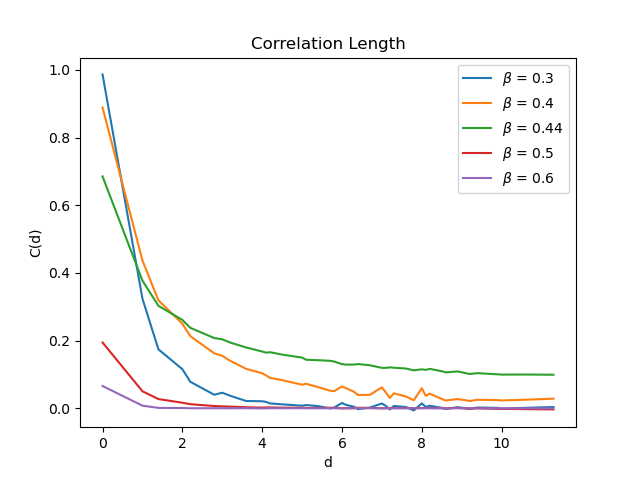
\includegraphics[width=\columnwidth]{plots/corr_len.png}
    \caption{Correlation Length}
    \label{fig:5}
\end{figure}
We see that at the critical point $\beta = 0.44$, the system exhibit much stronger correlations for large $d$ values
compared to other values at $\beta$. This is further evidence that the Ising model has a critical point at $\beta = 0.44$.
When $\beta$ is large, the spins are aligned together. This leads to high short range correlation but because the spins rarely fluctuate, 
they are stuck at their average value making the $\sigma - \langle \sigma \rangle$ small. At low $\beta$ the spins fluctuate chaotically 
leading to little correlation between spins. This emergent behavior of local interactions leading to long range communication has applications in
neuroscience where local interactions between nearby neurons leads to long range communication across distance areas of the brain.

The other property of criticality that we outlined in section 2.2 is scale invariance. 
Using DFS to count the size of each cluster, we plotted the distrubition of cluster sizes on the log-log plot. 
If the clusters have no characteristic scale, the distrubition of the cluster sizes follow a power law. 
On a log-log plot, power laws appear as straight lines. Plotting the distribution of cluster sizes for different
values of $\beta$ reveals that $\beta = 0.44$ gives a curve that resembles a straight line the most.

\begin{figure}[ht]
    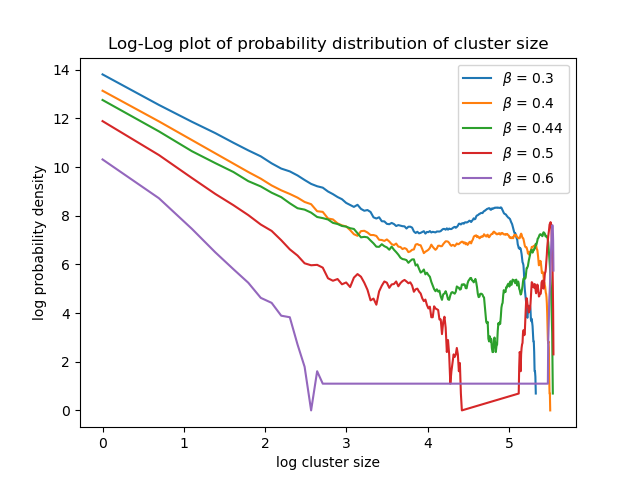
\includegraphics[width=\columnwidth]{plots/cluster_size.png}
    \caption{Distribution of cluster size}
    \label{fig:6}
\end{figure}

Although all of the curves start off straight but then get more chaotic as the cluster size increases, for $\beta = 0.44$
the linear relationship holds for the longest, up to clusters of size $\log 4$. We notice that as $\beta$ decreases, 
the frequency of small clusters increases. The chaotic behavior for large cluster sizes is likely due to the fact that the lattice
is not infinite and thus large clusters are overrepresented as they can loop around the lattice and form super large clusters. 
Furthermore, larger clusters are more rare making estimates for their frequency more noisy. 

At the critical point, many features of the Ising model follow power laws, not just the cluster size. Another example is
the correlation length. 

\begin{figure}[ht]
    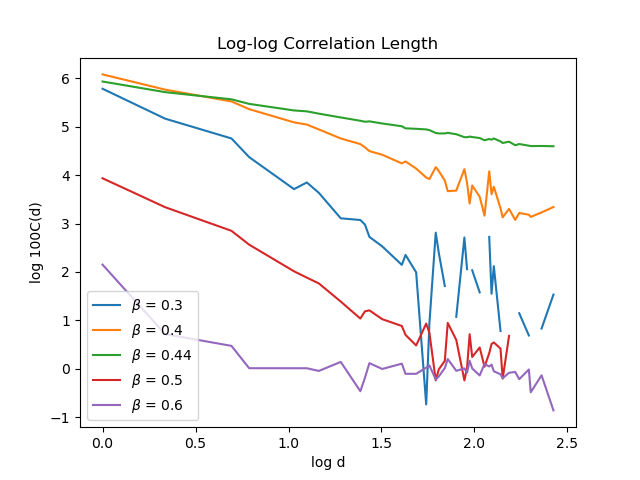
\includegraphics[width=\columnwidth]{plots/log_log_corr_len.png}
    \caption{Log-log plot of correlation length}
    \label{fig:6}
\end{figure}

As we can see at $\beta=0.44$, the correlation length on a log-log plot is a straight line, meaning it follows
a power law. Power laws are essential to understanding critical phenomenon. 


\section{Discussion}

\section{Conclusion}


\end{document}


% This document was modified from the file originally made available by
% Pat Langley and Andrea Danyluk for ICML-2K. This version was created
% by Iain Murray in 2018, and modified by Alexandre Bouchard in
% 2019 and 2021. Previous contributors include Dan Roy, Lise Getoor and Tobias
% Scheffer, which was slightly modified from the 2010 version by
% Thorsten Joachims & Johannes Fuernkranz, slightly modified from the
% 2009 version by Kiri Wagstaff and Sam Roweis's 2008 version, which is
% slightly modified from Prasad Tadepalli's 2007 version which is a
% lightly changed version of the previous year's version by Andrew
% Moore, which was in turn edited from those of Kristian Kersting and
% Codrina Lauth. Alex Smola contributed to the algorithmic style files.
